\section{All Things were restored to Order}

\begin{figure}[h]\centering
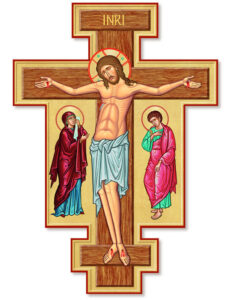
\includegraphics[width=.25\textwidth]{ChristOrans-237x300.jpg}
\end{figure}

\begin{quotex}
The day, eternally joyous and sad, the Son of God Made Man was placed on a cross, all things at once were restored to order, and in that divine order the cross was raised above all things created. Some of these manifested the goodness of God, some His mercy, others His justice.

The cross alone was the symbol of His love and the pledge of His grace. Through it the confessors confessed, and the virgins were chaste, and the fathers of the desert led angelic lives, and the martyrs were firm witnesses who laid down their lives with manly and unshaken constancy. From the sacrifice of the cross proceeded that marvelous energy with which the weak astounded the strong, the proscribed and disarmed ascended the Capitol, and some poor fishermen conquered the world.

Through the cross all who conquer gain victory; all who combat, strength; all who seek it, mercy; the unprotected, protection; those who are sad, joy; and consolation, all who weep. Since the cross was raised in the air there is no man who cannot live in heaven before his mortal remains are consigned to the earth; for if he lives here in tribulation, he lives there in hope.
\flright{\textsc{Donoso Cortes}}
\end{quotex}



\flrightit{Posted on 2010-04-02 by Cologero}

